\documentclass[../main.tex]{subfiles}

\subsection{Interferenz}
\begin{frame}
    \frametitle{Grundlagen}
    \framesubtitle{Interferenz}
    \begin{figure}[ht]
        \begin{subfigure}[b]{0.35\textwidth}
            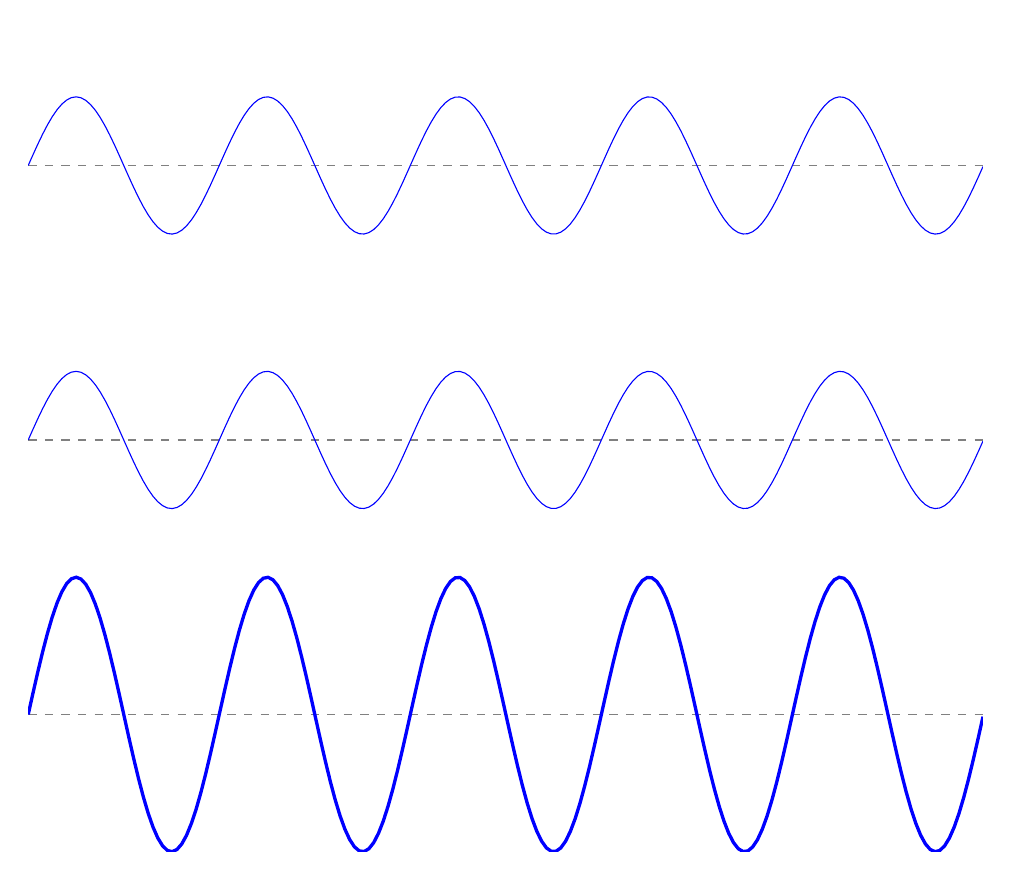
\begin{tikzpicture}
            \begin{axis}[
                xmin=0,xmax=31.4,
                ymin=-3,ymax=3,
                ticks=none,
                axis line style=white,
                scale only axis,
                domain=0:31.4,
                width=\textwidth,
            ]
                \addplot[gray,dashed,thin]{2};
                \addplot[samples=200,blue] {sin(deg(x))/2+2};
                \addplot[gray,dashed,thin]{0};
                \addplot[samples=200,blue] {sin(deg(x))/2};
                \addplot[gray,dashed,thin]{-2};
                \addplot[samples=200,blue,very thick] {sin(deg(x))-2};
            \end{axis}
            \end{tikzpicture}
        \end{subfigure}
        \hspace{0.5cm}
        \begin{subfigure}[b]{0.35\textwidth}
            \begin{tikzpicture}
            \begin{axis}[
                xmin=0,xmax=31.4,
                ymin=-3,ymax=3,
                ticks=none,
                axis line style=white,
                scale only axis,
                domain=0:31.4,
                width=\textwidth,
            ]
                \addplot[gray,dashed,thin]{2};
                \addplot[samples=200,blue] {sin(deg(x+3.14))/2+2};
                \addplot[gray,dashed,thin]{0};
                \addplot[samples=200,blue] {sin(deg(x))/2};
                \addplot[gray,dashed,thin]{-2};
                \addplot[samples=200,blue,very thick] {-2};
            \end{axis}
            \end{tikzpicture}
        \end{subfigure}
    \end{figure}
\end{frame}

\subsection{Doppelspaltexperiment}
\begin{frame}
    \frametitle{Grundlagen}
    \framesubtitle{Doppelspaltexperiment}
\end{frame}

\subsection{Absorption}
\begin{frame}
    \frametitle{Grundlagen}
    \framesubtitle{Absorption}
\end{frame}